\documentclass[a4paper,14pt]{extarticle}
\usepackage{../../tex-shared/report-layout}

\renewcommand{\mylabnumber}{5}
\renewcommand{\mylabtitle}{Планирование проекта}
\renewcommand{\mysubject}{Управление IT-проектами}
\renewcommand{\mylecturer}{Смирнова Н.Б.}

\begin{document}
\begin{titlepage}
    
    \thispagestyle{empty}
    
    \begin{center}
        
        Министерство науки и Высшего образования Российской Федерации \\
        Севастопольский государственный университет \\
        Кафедра ИС
        
        \vfill

        Отчет \\
        по лабораторной работе №\mylabnumber \\
        \enquote{\mylabtitle} \\
        по дисциплине \\
        \enquote{\MakeTextUppercase{\mysubject}}

    \end{center}

    \vspace{1cm}

    \noindent\hspace{7.5cm} Выполнил студент группы ИС/б-17-2-о \\
    \null\hspace{7.5cm} Горбенко К. Н. \\
    \null\hspace{7.5cm} Проверил \\
    \null\hspace{7.5cm} \mylecturer

    \vfill

    \begin{center}
        Севастополь \\
        \the\year{}
    \end{center}

\end{titlepage}

\section{Цель работы}
Освоить навыки планирования проекта.

\section{Задание на работу}
\begin{enumerate}
    \item Составить одностраничное описание проекта.
    \item Написать ИСР (WBS) проекта.
    \item Назначить исполнителей на каждую работу.
    \item С учетом только заработной платы/ставки в час каждого из исполнителей рассчитать примерную стоимость проекта.
\end{enumerate}

\begin{table}[H]
    \caption{Общая информация о проекте}
    \begin{tabular}{ | p{5.5cm} | p{11cm} | }
        \hline
        Наименование проекта & Разработка адаптивного сервиса для изучения иностранной лексики \\ \hline
        Краткое наименование проекта & Разработка адаптивного сервиса для изучения иностранной лексики \\ \hline
        Заказчик проекта & Севастопольский государственный университет \\ \hline
        Дата начала проекта & 01.03.2021 \\ \hline
        Дата окончания проекта & 31.06.2021 \\ \hline
    \end{tabular}
\end{table}

\section{Ход работы}
\subsection{Описание проекта}
\begin{table}[H]
    \caption{Описание проекта}
    \begin{tabular}{ | p{5.5cm} | p{11cm} | }
        \hline
        Название проекта & Адаптивного сервиса для изучения иностранной лексики \\ \hline
        Предметная область & Лексика иностранного языка \\ \hline
        Вид проекта по характеру деятельности & Технический (разработка программного обеспечения) \\ \hline
        Класс проекта & Монопроект (отдельный проект) \\ \hline
        Вид проекта & Инновационный (разработка новой технологии) \\ \hline
        Длительность & Краткосрочный (до 3-х лет) \\ \hline
        Проблемы & 1. Невозможно обращаться к источникам на иностранном языке не владея достаточным объемом лексики \linebreak
                   2. Лексика, изученная при обращении к источникам, быстро забывается \linebreak
                   3. При изучении лексики нужно изучать также и варианты ее
                   использования, контексты, в которых она может использоваться \\ \hline
        Цель & Создать адаптивный сервис для изучения иностранной лексики, который позволил бы решить вышеизложенные проблемы \\ \hline
        Задачи проекта & 1. Исследовать область изучения иностранной лексики \linebreak
                         2. Разработать алгоритмы выявления очередной лексической единицы для проверки пользователя \linebreak
                         3. Разработать алгоритм упражнений \linebreak
                         4. Разработать с помощью полученных алгоритмов систему для изучения иностранной лексики \\ \hline
        Ожидаемый результат & Сайт для изучения иностранной лексики \\ \hline
    \end{tabular}
\end{table}

Данная система является актуальной т.к. большинство информации в мире находится
в языке оригинала. По сравнению с другими сервисами данная система позволит
изучать лексику таким образом, чтобы она не только не забывалась со временем, но
и могла использоваться в повседневной жизни (при общении).

\subsection{ИСР (WBS) проекта}
\begin{figure}[H]
    \centering
    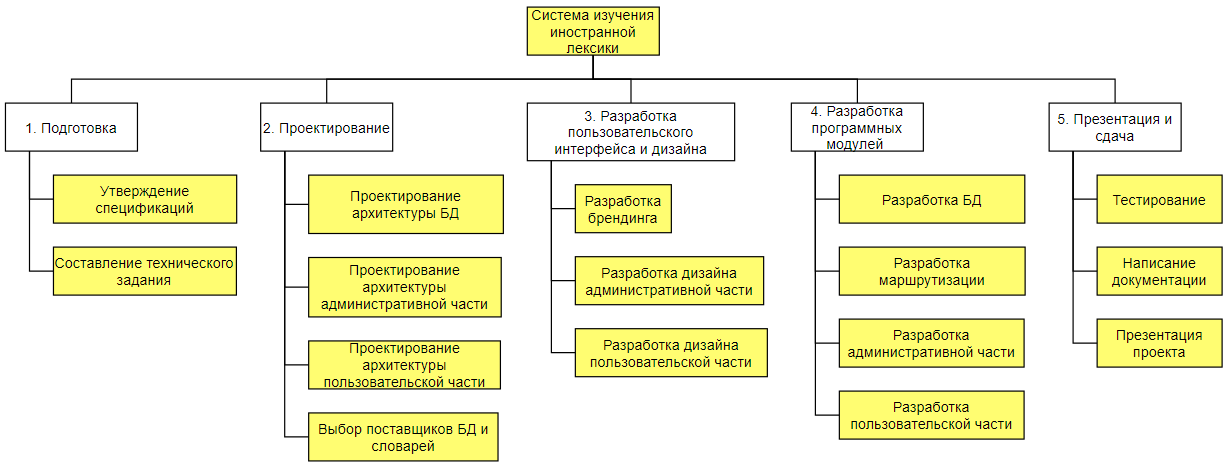
\includegraphics[width=\linewidth]{wbs}
    \caption{WBS проекта}
    \label{fig:wbs}
\end{figure}

\subsection{Исполнители проекта}
\begin{table}[H]
    \caption{Исполнители проекта}
    \begin{tabular}{ | p{3cm} | p{3.5cm} | p{2cm} | p{7cm} | }
        \hline
        ФИО & Специализации & Ставка & Задачи \\ \hline
        Горбенко К.Н. & Менеджер & 1000 & Организация, планирование, презентация \\ \hline
        Васильев И.А & Архитектор & 1500 & разработка БД, разработка маршрутизации \\ \hline
        Иванов И.И. & Разработка & 1200 & разработка административной части, разработка пользовательской части \\ \hline 
        Фетисов В.Д. & Дизайн & 1300 & Разработка общего брендинга \\ \hline
        Брыкова Е.Н. & Тестирование & 700 & Тестирование базы данных, тестирование административной частит, тестирование пользовательской части, тестирование полной системы \\ \hline
        Жукова А.П. & Дизайн & 600 & Разработка дизайна административной части, разработка дизайна пользовательской части \\ \hline
    \end{tabular}
\end{table}

\subsection{Стоимость затрат}
\begin{figure}[H]
    \centering
    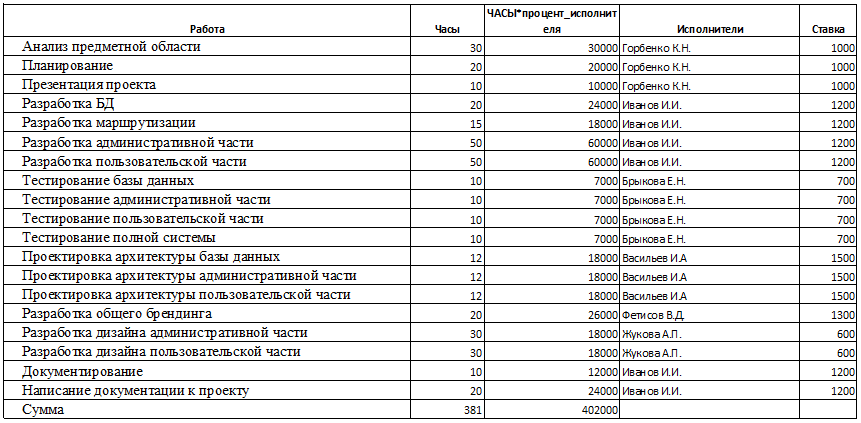
\includegraphics[width=\linewidth]{salaries1}
    \caption{Расходы}
    \label{fig:salaries1}
\end{figure}

\begin{figure}[H]
    \centering
    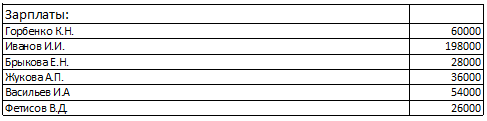
\includegraphics[width=\linewidth]{salaries2}
    \caption{Зарплаты}
    \label{fig:salaries2}
\end{figure}

\section*{Выводы}
В ходе лабораторной работы были освоены навыки планирования проекта. Был
составлен бюджет проекта на основе зароботных плат его участников.

\end{document}